%%%%%%%%%%%%%%%%%%%%%%%%%%%%%%%%%%%%%%%%%
% Tufte Essay
% LaTeX Template
% Version 2.0 (19/1/19)
%
% This template originates from:
% http://www.LaTeXTemplates.com
%
% Authors:
% The Tufte-LaTeX Developers (https://www.ctan.org/pkg/tufte-latex)
% Vel (vel@LaTeXTemplates.com)
%
% License:
% Apache License, version 2.0
%
%%%%%%%%%%%%%%%%%%%%%%%%%%%%%%%%%%%%%%%%%

%----------------------------------------------------------------------------------------
%	PACKAGES AND OTHER DOCUMENT CONFIGURATIONS
%----------------------------------------------------------------------------------------

\documentclass[a4paper]{tufte-handout} % Use A4 paper by default, remove 'a4paper' for US letter

\usepackage{graphicx} % Required for including images
\setkeys{Gin}{width=\linewidth, totalheight=\textheight, keepaspectratio} % Default images settings
\graphicspath{{Figures/}{./}} % Specifies where to look for included images (trailing slash required)

\usepackage{amsmath, amsfonts, amssymb, amsthm} % For math equations, theorems, symbols, etc
\usepackage{units} % Non-stacked fractions and better unit spacing

\usepackage{booktabs} % Required for better horizontal rules in tables
\usepackage{subfigure}
\usepackage{parskip}

%----------------------------------------------------------------------------------------
%	TITLE SECTION
%----------------------------------------------------------------------------------------

\title{Audio Program Design and Application - 6}

\author{Chuhan Qiu}


%----------------------------------------------------------------------------------------

\begin{document}

\maketitle % Print the title section

%----------------------------------------------------------------------------------------
%	ABSTRACT/SUMMARY
%----------------------------------------------------------------------------------------

\begin{abstract}
	\textbf{Summary}
In this report, I use the equalizer which implemented in my final project of last term,
to filter audio signal using different filter curve, including peak filters and shelf filters(pass filter can also be implemented using shelf filter with maximum attenuation).
When I designed the equalizer, I joined in many curve preset, which makes the set of combination of peak filter, shelf filter and pass filter very convenient.
Besides, I design an all-pass filter which implements the phase compensation to first/second order low-pass filter.
\end{abstract}

%----------------------------------------------------------------------------------------
%	ESSAY BODY
%----------------------------------------------------------------------------------------

\section{Previous Research}
Equalizer, which is actually the most basic and important audio effect in audio signal processing, can be implemented easily through combining several different types of first/second-order filters. In DAFX\footnote{Udo Zölzer, 2011, DAFX: Digital Audio Effects, /10.1002/9781119991298}, Zölzer has introduced most types of first/second-order filter designing methods and formulas. And in my final project of last term, I designed the equalizer in Figure 1 based on the methods and formulas given by DAFX.

\begin{figure}[h]
	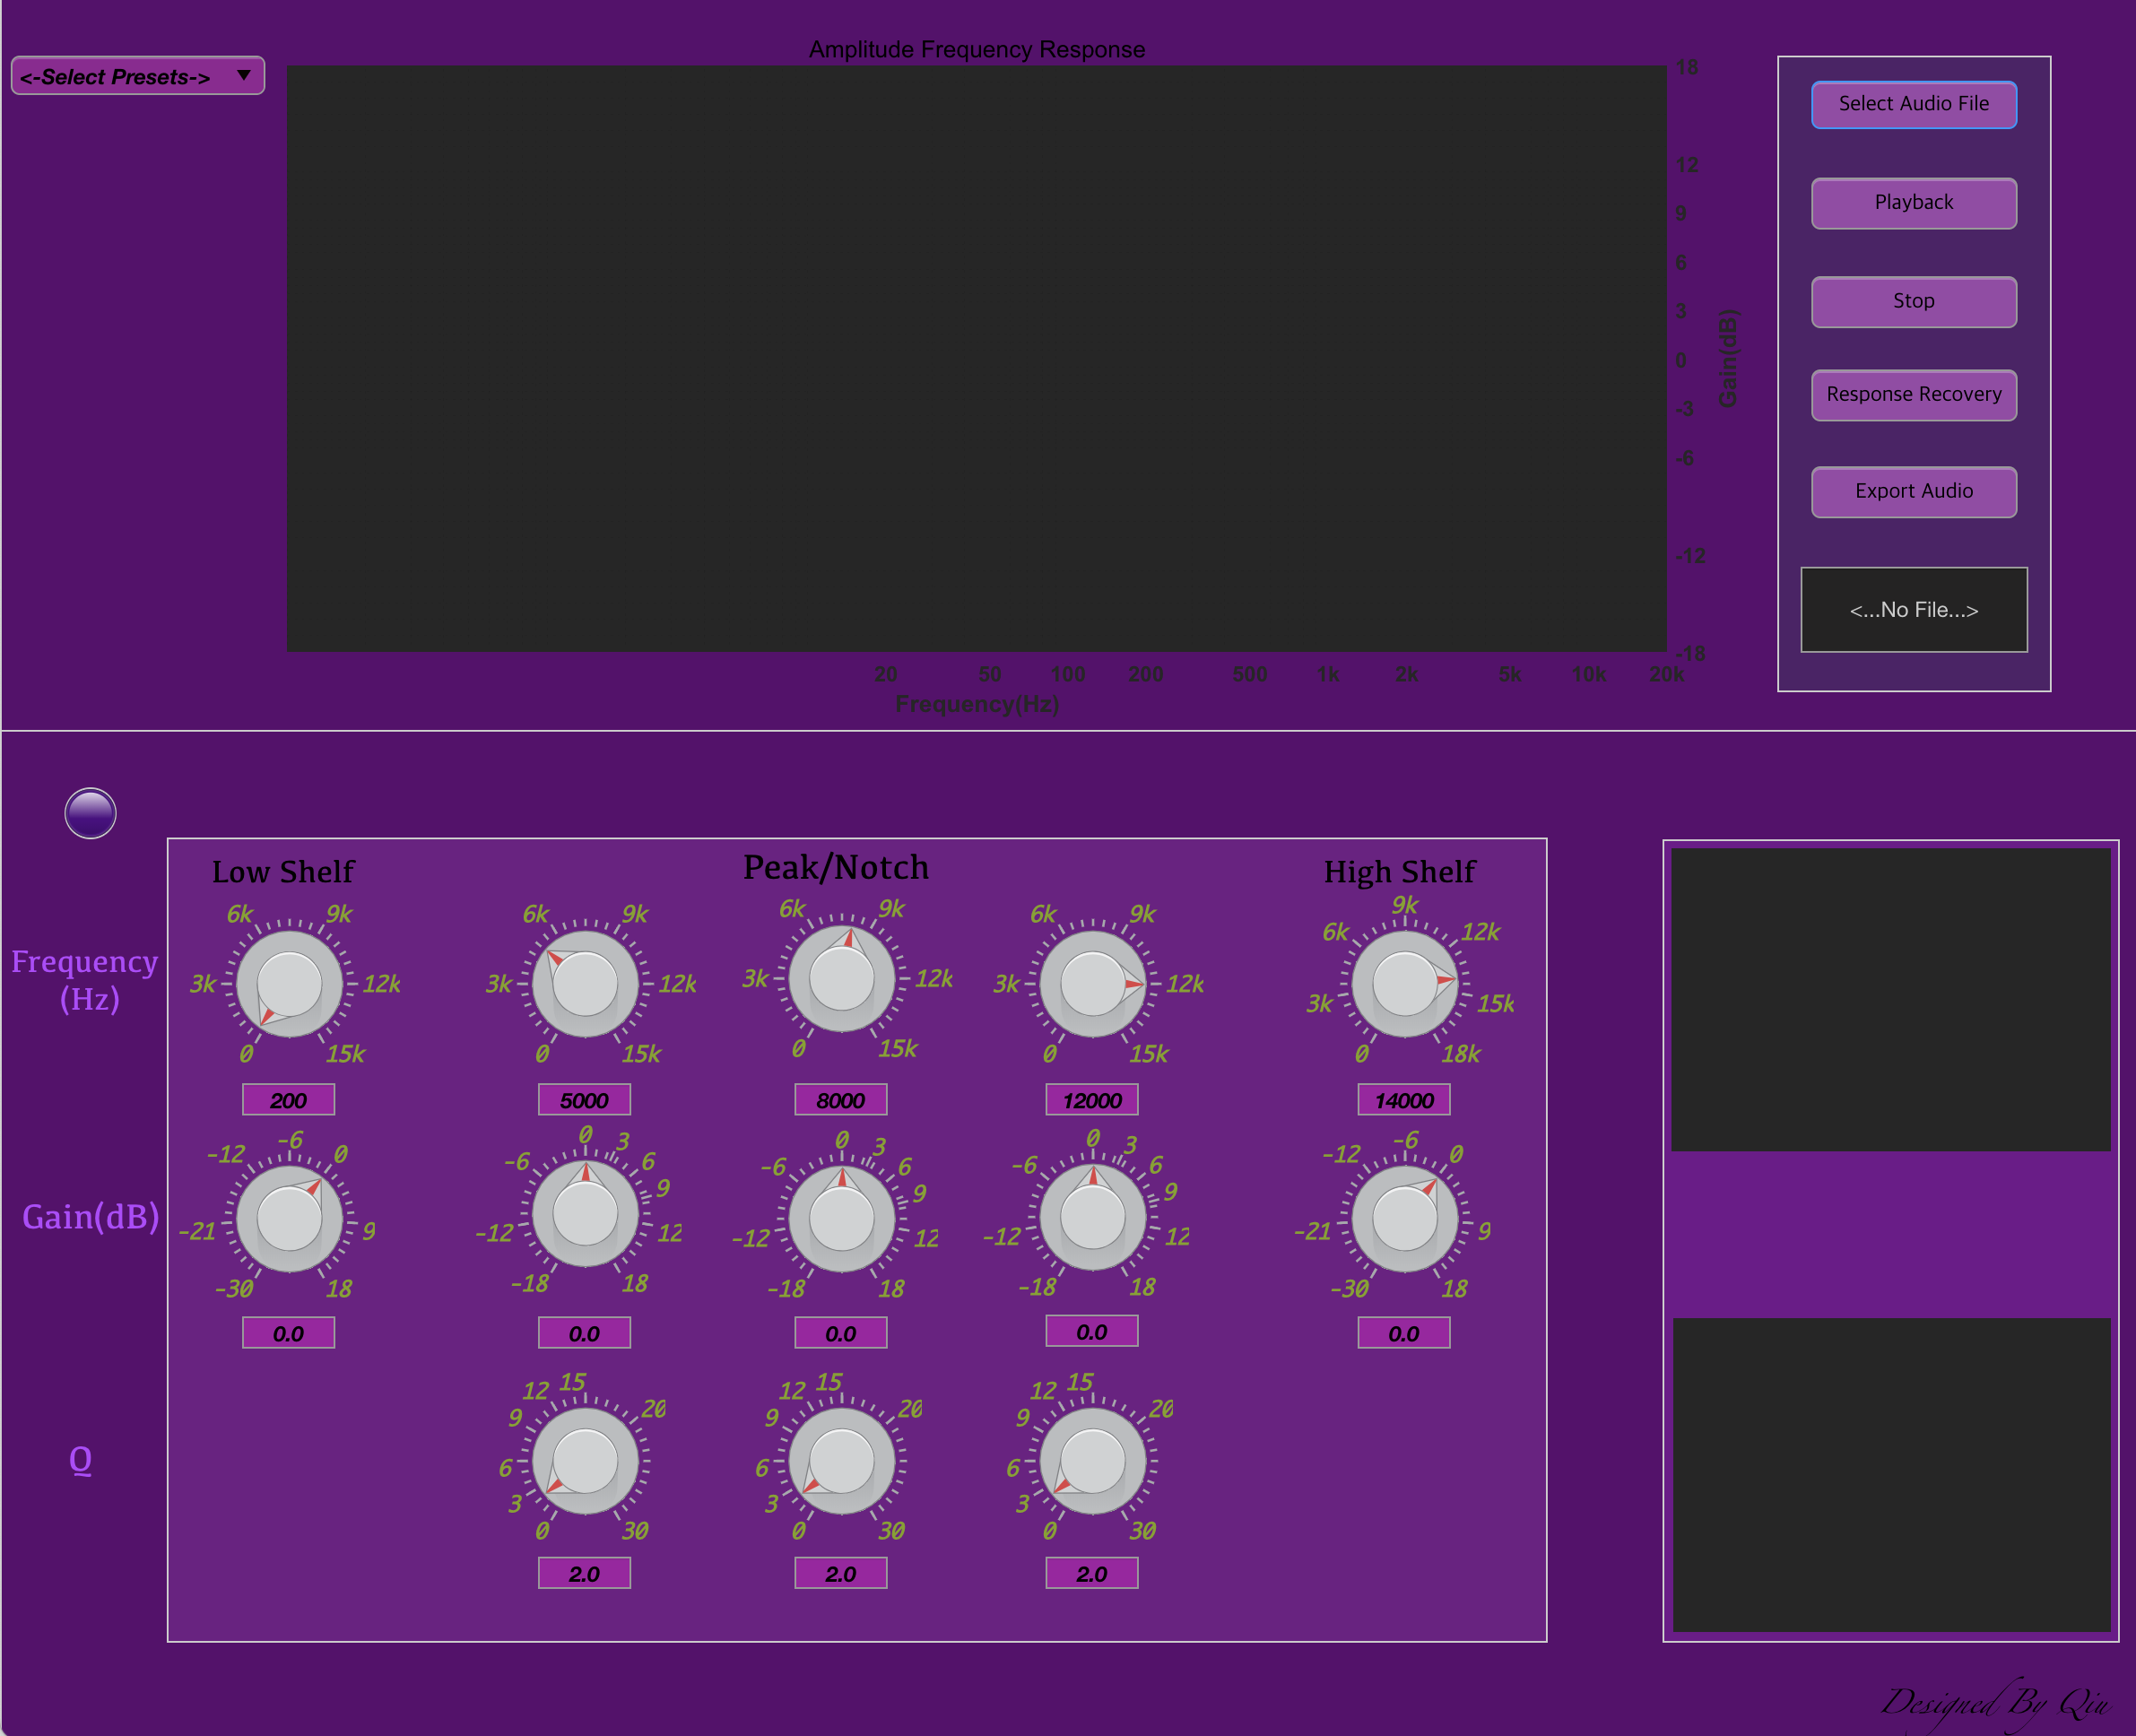
\includegraphics{Image/Filter.png}
	\caption{The UI of equalizer designed by myself}
	\label{fig:textfig}
	\setfloatalignment{a} % Position the figure caption in the middle of the figure
\end{figure}

As Figure 1, the equalizer has three peak filters and two shelf filters. By adjusting the gain of them, it is able to create an approximate pass filter. In this way, we can use this equalizer to make the sound more expressive and filter unneeded frequency components. In the top left corner, there are many presets for us to choose, which can also provides special processing and effect to the sound.

In my final project's report of last term, I raised the question of how to implement phase compensation to IIR filters. At that time, I analyzed it from the perspective of Z-plane, and proved that there is non-existent strict phase compensation because of the specific structure of IIR. We know that FIR filter is linear phase response and no matter what order is it, its poles are all distributed at the origin. So many people assert that whether the filter is linear phase response depends on the pole distribution. However, this viewpoint actually falls into the trap. After searching for information from different sources and verifying, the linear phase response filter must meet the condition in equation (1).
\begin{equation}
\frac{1}{z_i}=\frac{z_j^*}{|z_j|^2}
\end{equation}

where $z_i$ and $z_j$ refer to a pair of zeros or poles in the Z-plane of linear phase response filter. Commonly, for strictly linear phase response filter, both the zeros and poles of it must be distributed in pairs with respect to the conjugate symmetry of the unit circle in Z-plane. However, the pole distribution of IIR filter determines that it cannot meet the condition in equation (1). The poles of IIR filter appear anywhere within the unit circle of Z-plane, and their conjugate symmetric poles will absolutely distribute outside the unit circle which makes the system no longer stable.

So we can only approximate the phase compensation of IIR filter. And the method I proposed includes following steps:
\begin{enumerate}
    \item Connect the phase response of IIR filter at zero and Nyquist frequency;
    \item Calculate the difference between the linear line and original phase response;
    \item Take the difference curve as the phase response, design all-pass filter and compensate the IIR filter.
\end{enumerate}

\section{Equalizer Setup}
The equalizer designed by myself was implemented in AppDesigner, which is a Matlab native interaction application development tool. The function description for the equalizer is shown as Figure (2).
\begin{figure}[h]
    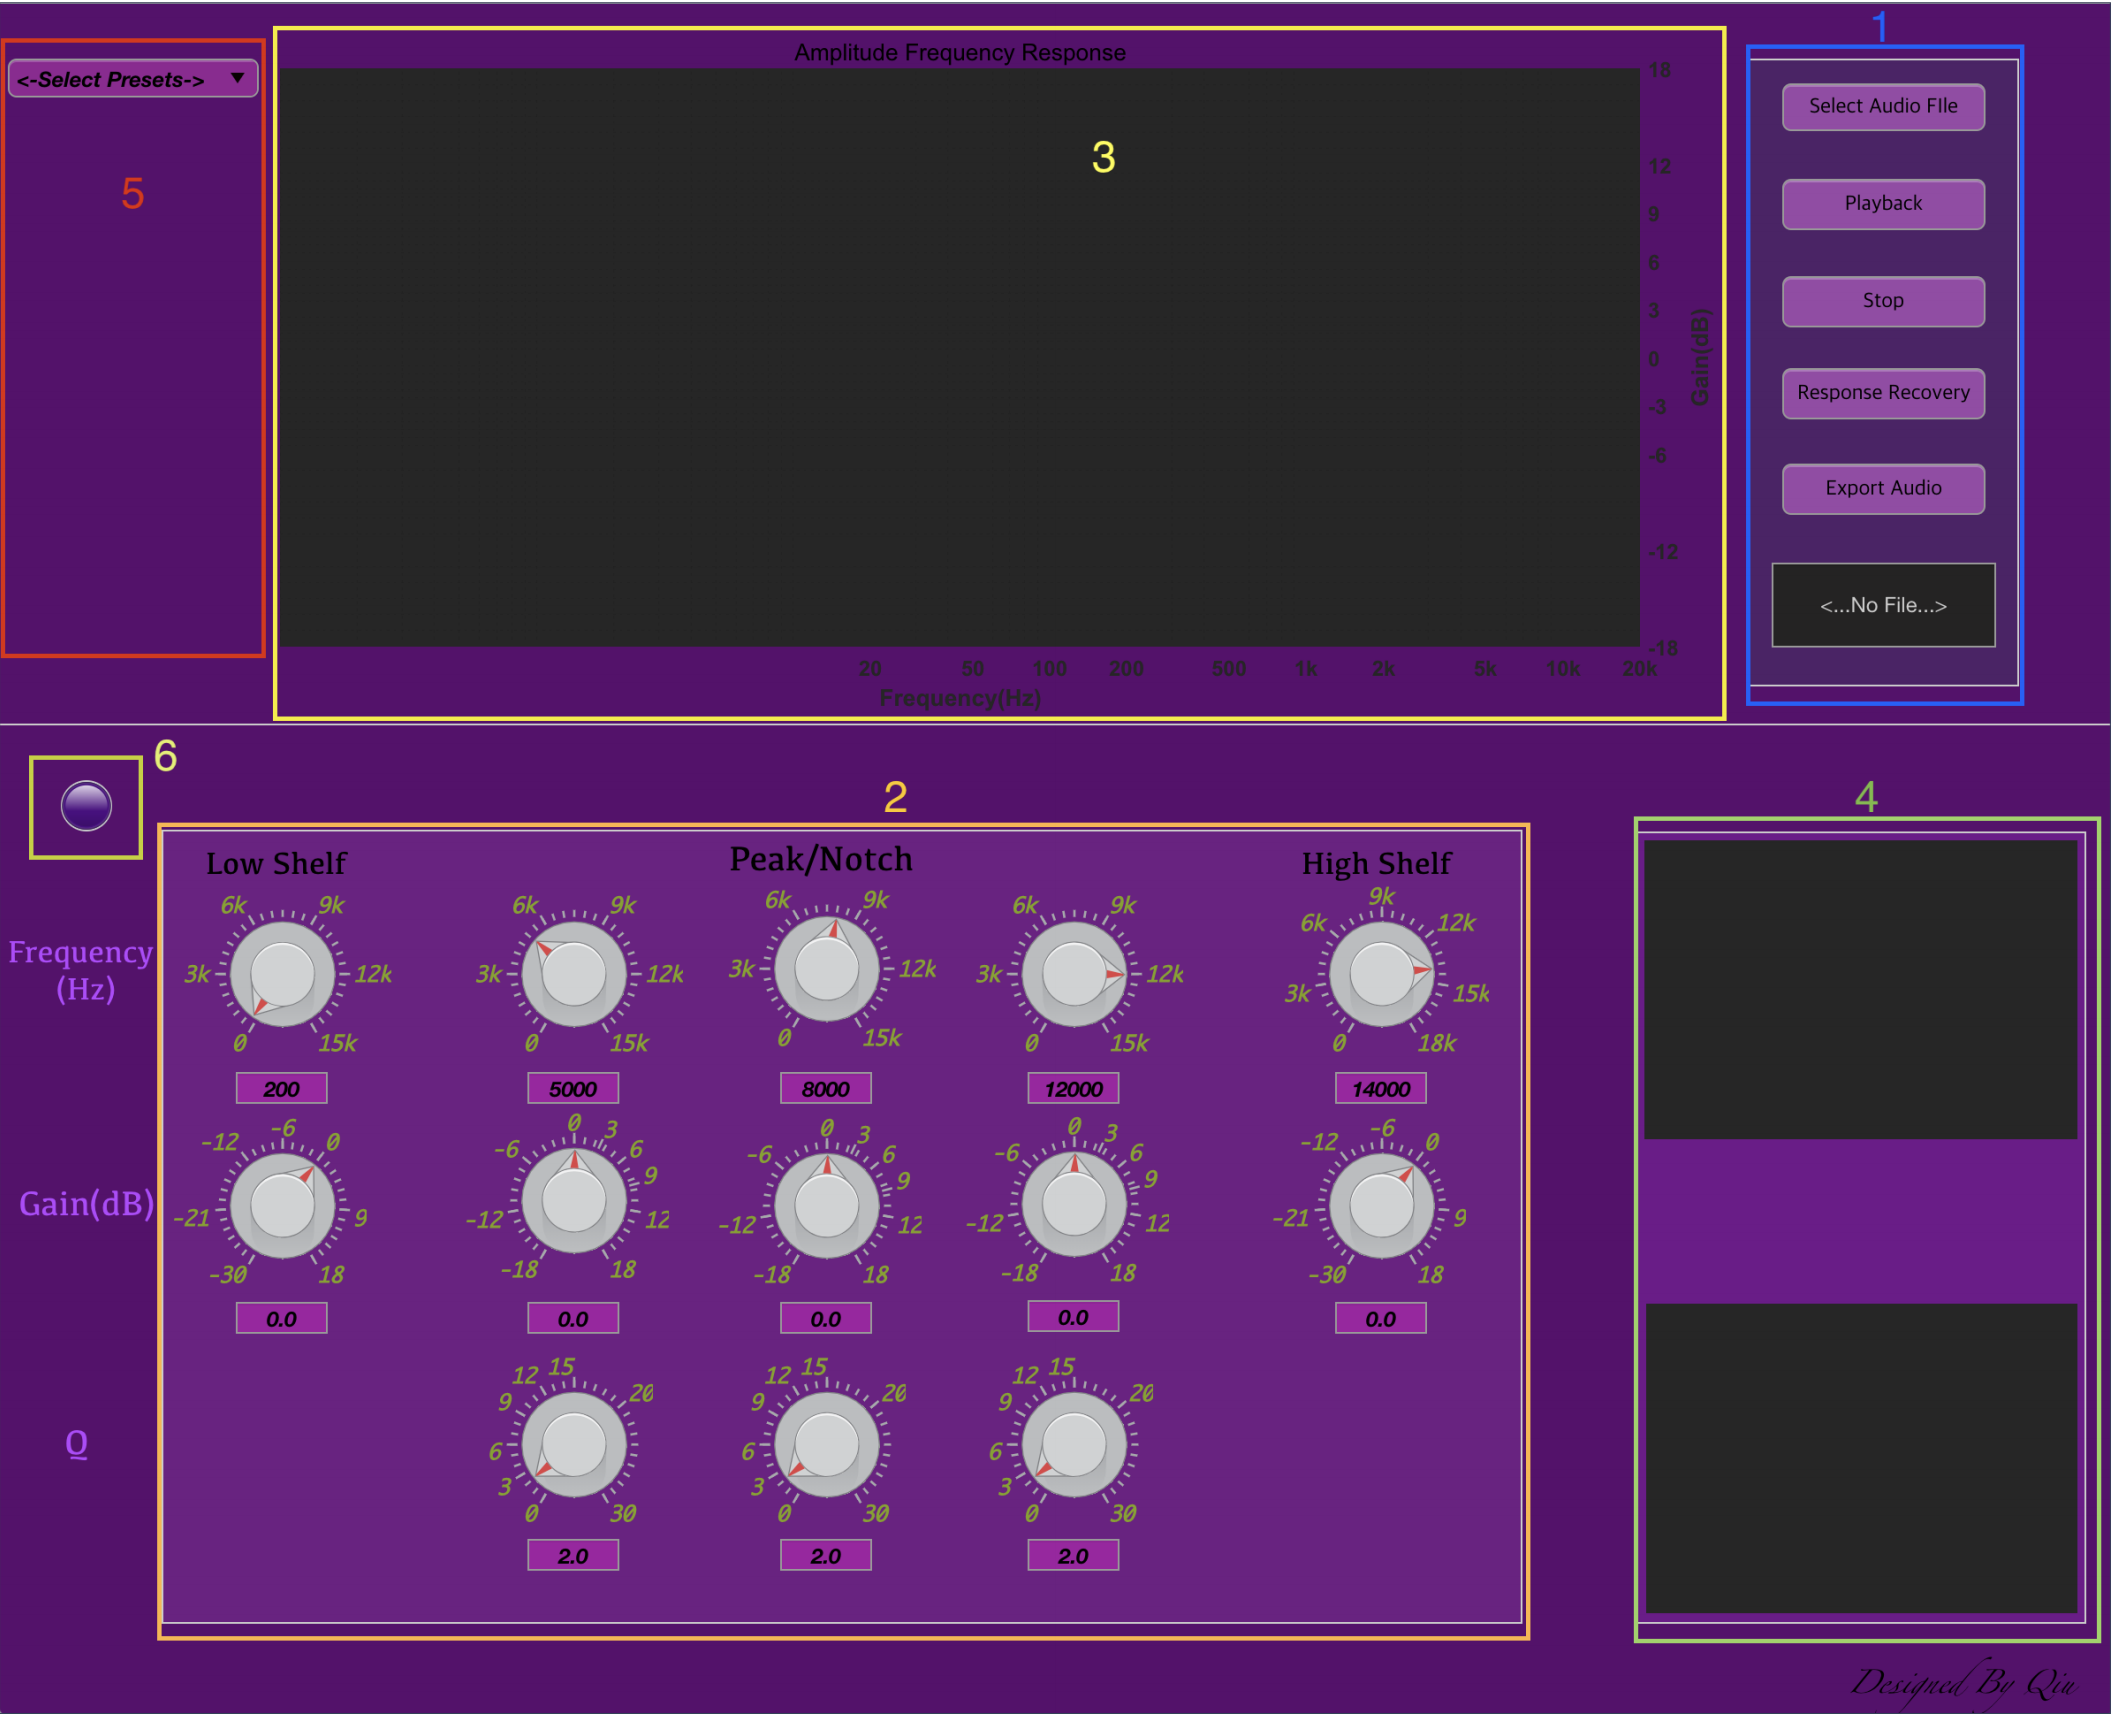
\includegraphics{Image/FilterRefer.png}
    \caption{Function zoning}
    \label{fig:textfig}
	\setfloatalignment{a} % Position the figure caption in the middle of the figure
\end{figure}
\begin{enumerate}
    \item Import, export, playback and stop of audio file.'Response Recovery' can initialize the frequency response.
    \item Adjust the parameters of equalizer, including cut-off/center frequency, gain and band width.
    \item Display the curve of frequency response.
    \item The original spectrogram(above) and the filtered spectrogram(below).
    \item Presets selection, totally 11 presets are available for selection.
    \item The promote signal light of updating the spectrogram.
\end{enumerate}

I use an audio signal which contain two parts: piano and string. In my opinion, this music segment's predominant instrument should be string because the melody lines of string is much richer than piano and string may contain more emotions. However, the piano part contains too much low-frequency, which makes it take the dominant position. Especially for the parts below 200 Hz, so this music segment's frequency structure is actually out of balance. 
In this way, I wanna filter these low-frequency components to make the music segment more balanced. I set the low shelf filter's cut-off frequency at 200 Hz and gain at -30 dB. Then the frequency response of equalizer in Figure 3 (a) looks the same as a high-pass filter. Although I filter the low frequency of it, the current status of string is still not prominent enough. Through the analyzation of music segment's spectrogram, the main frequency range of string is actually above 1.2 kHz, so I try to set the gain at 1.5 kHz to +3 dB and 3 kHz to +4.5 dB as Figure 3 (b). The significance degree of string and the balance of the instruments as a whole has increased a lot.  
Next, I want to show the effect of two interesting equalizer presets. The preset 'Phone', which is as shown in Figure 3 (c), has a large gain at mid-frequency, while cut-off most high-frequency and low-frequency components, to provide a telephone sound effect. Telephone sound effect is a widely used audio effect in film sound production. Then, I select 'Above Enhance(Shu-Nung)' preset, which is based on the research of Shu-Nung and Li Jen\footnote{Yao, Shu-Nung, and Li Jen Chen. HRTF Adjustments with Audio Quality Assessments. Archives of Acoustics, Mar. 2013. De Gruyter, https://doi.org/10.2478/aoa-2013-0007.}. Because of the low-frequency characteristic of the audio signal, I set a low-cut to it based on the preset 'Above Enhance'. After filtering by this above enhancement curve, I can slightly feel the source of the sound shift to upward a little bit, which is pretty interesting. 
\begin{figure}[h!]
    \centering
    \subfigure[First step]{
        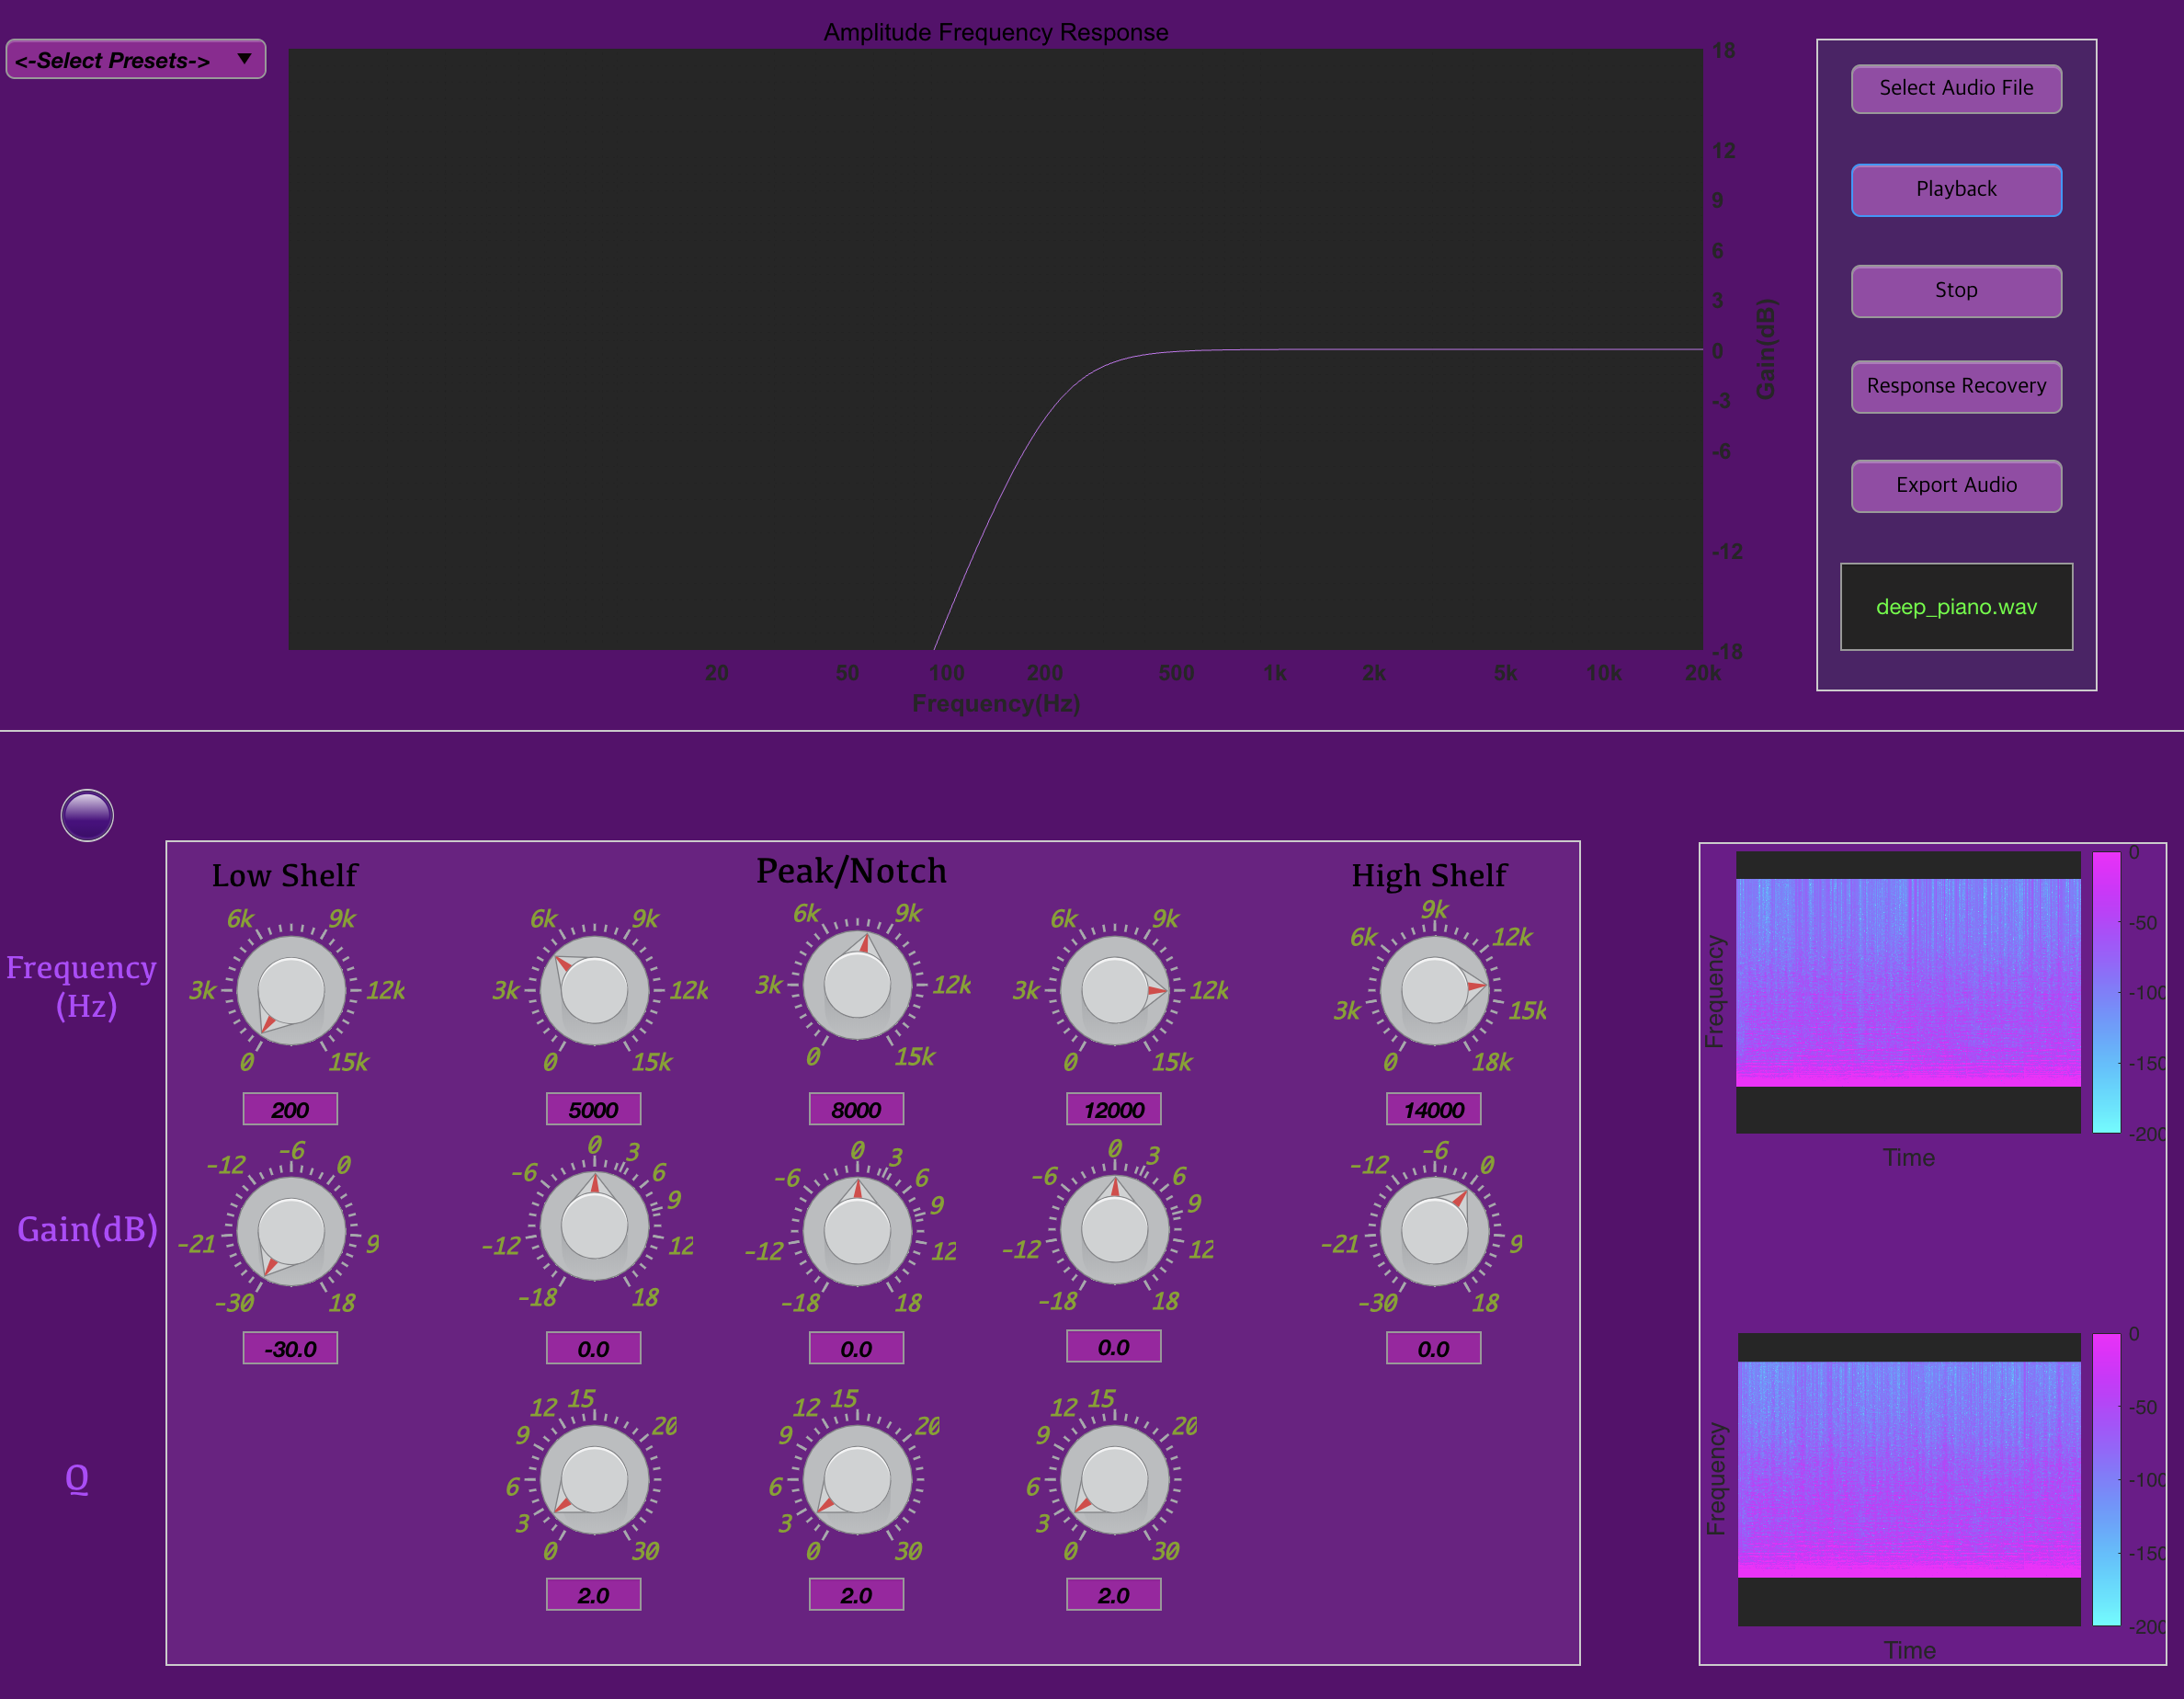
\includegraphics[width=2in]{Image/200HzLowCut.png}
    }
    \subfigure[Second step]{
	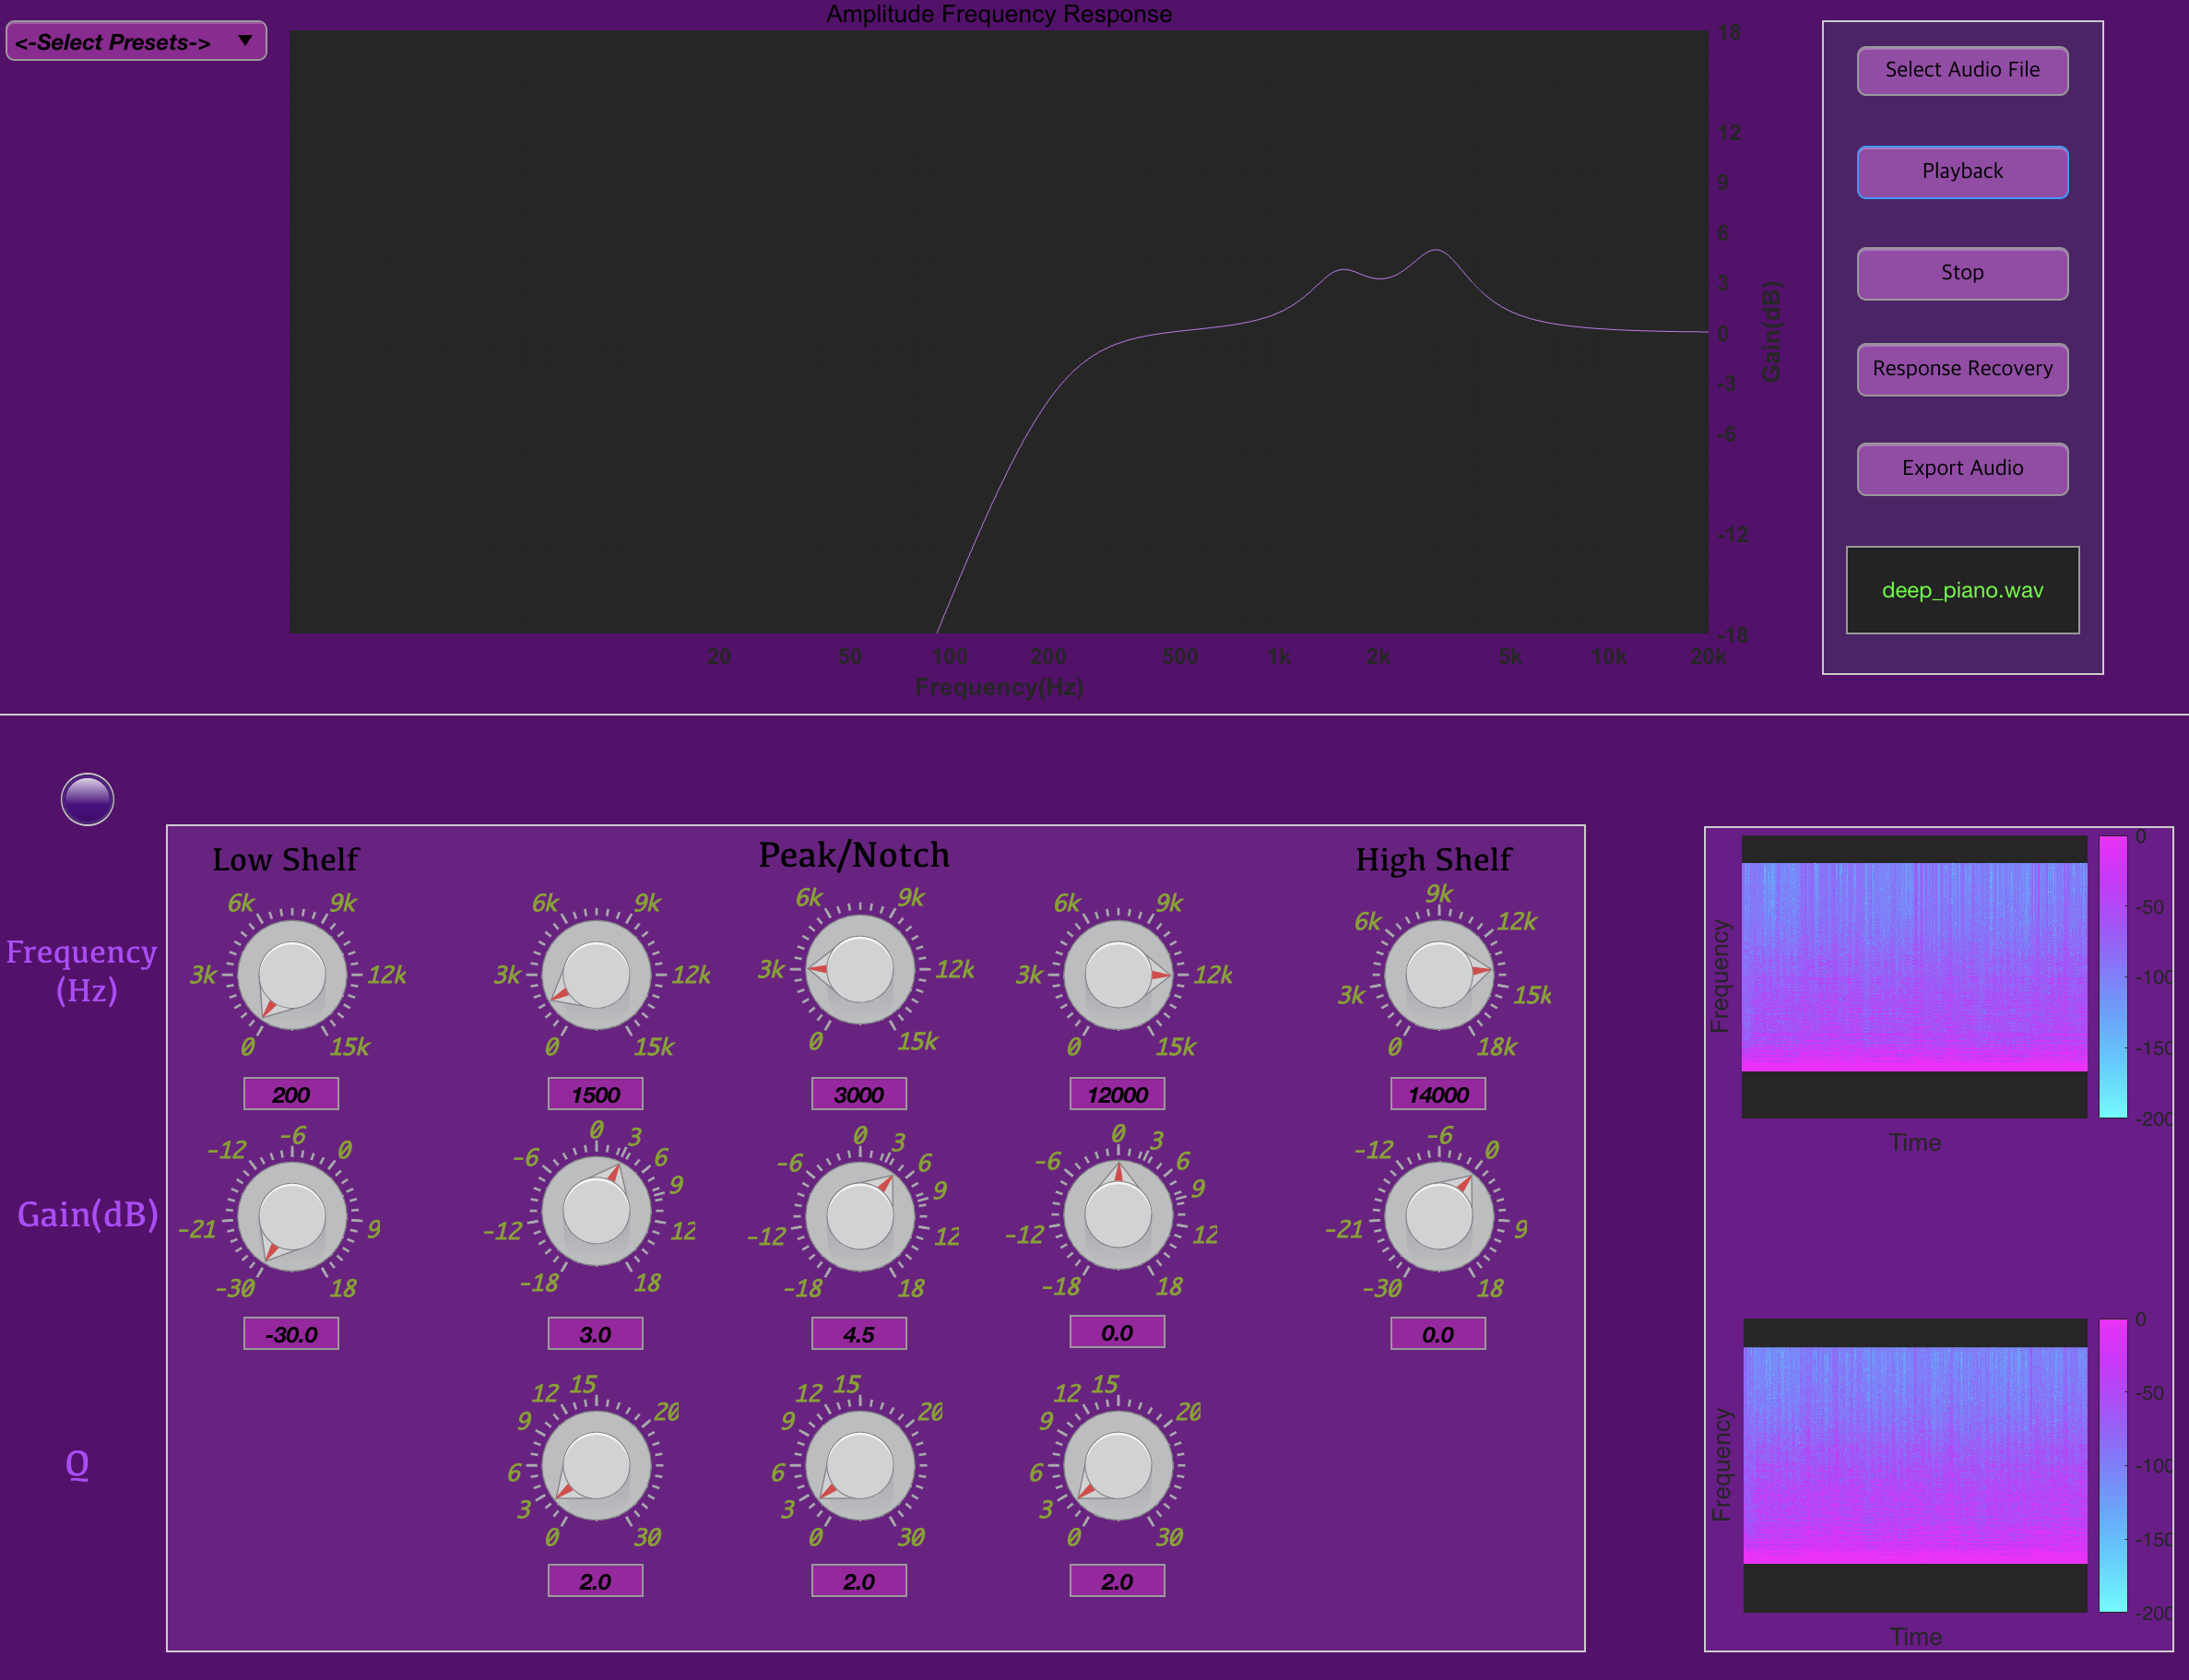
\includegraphics[width=2in]{Image/1500_2000Peak.png}
    }
    \\
    \subfigure['Phone' preset]{
    	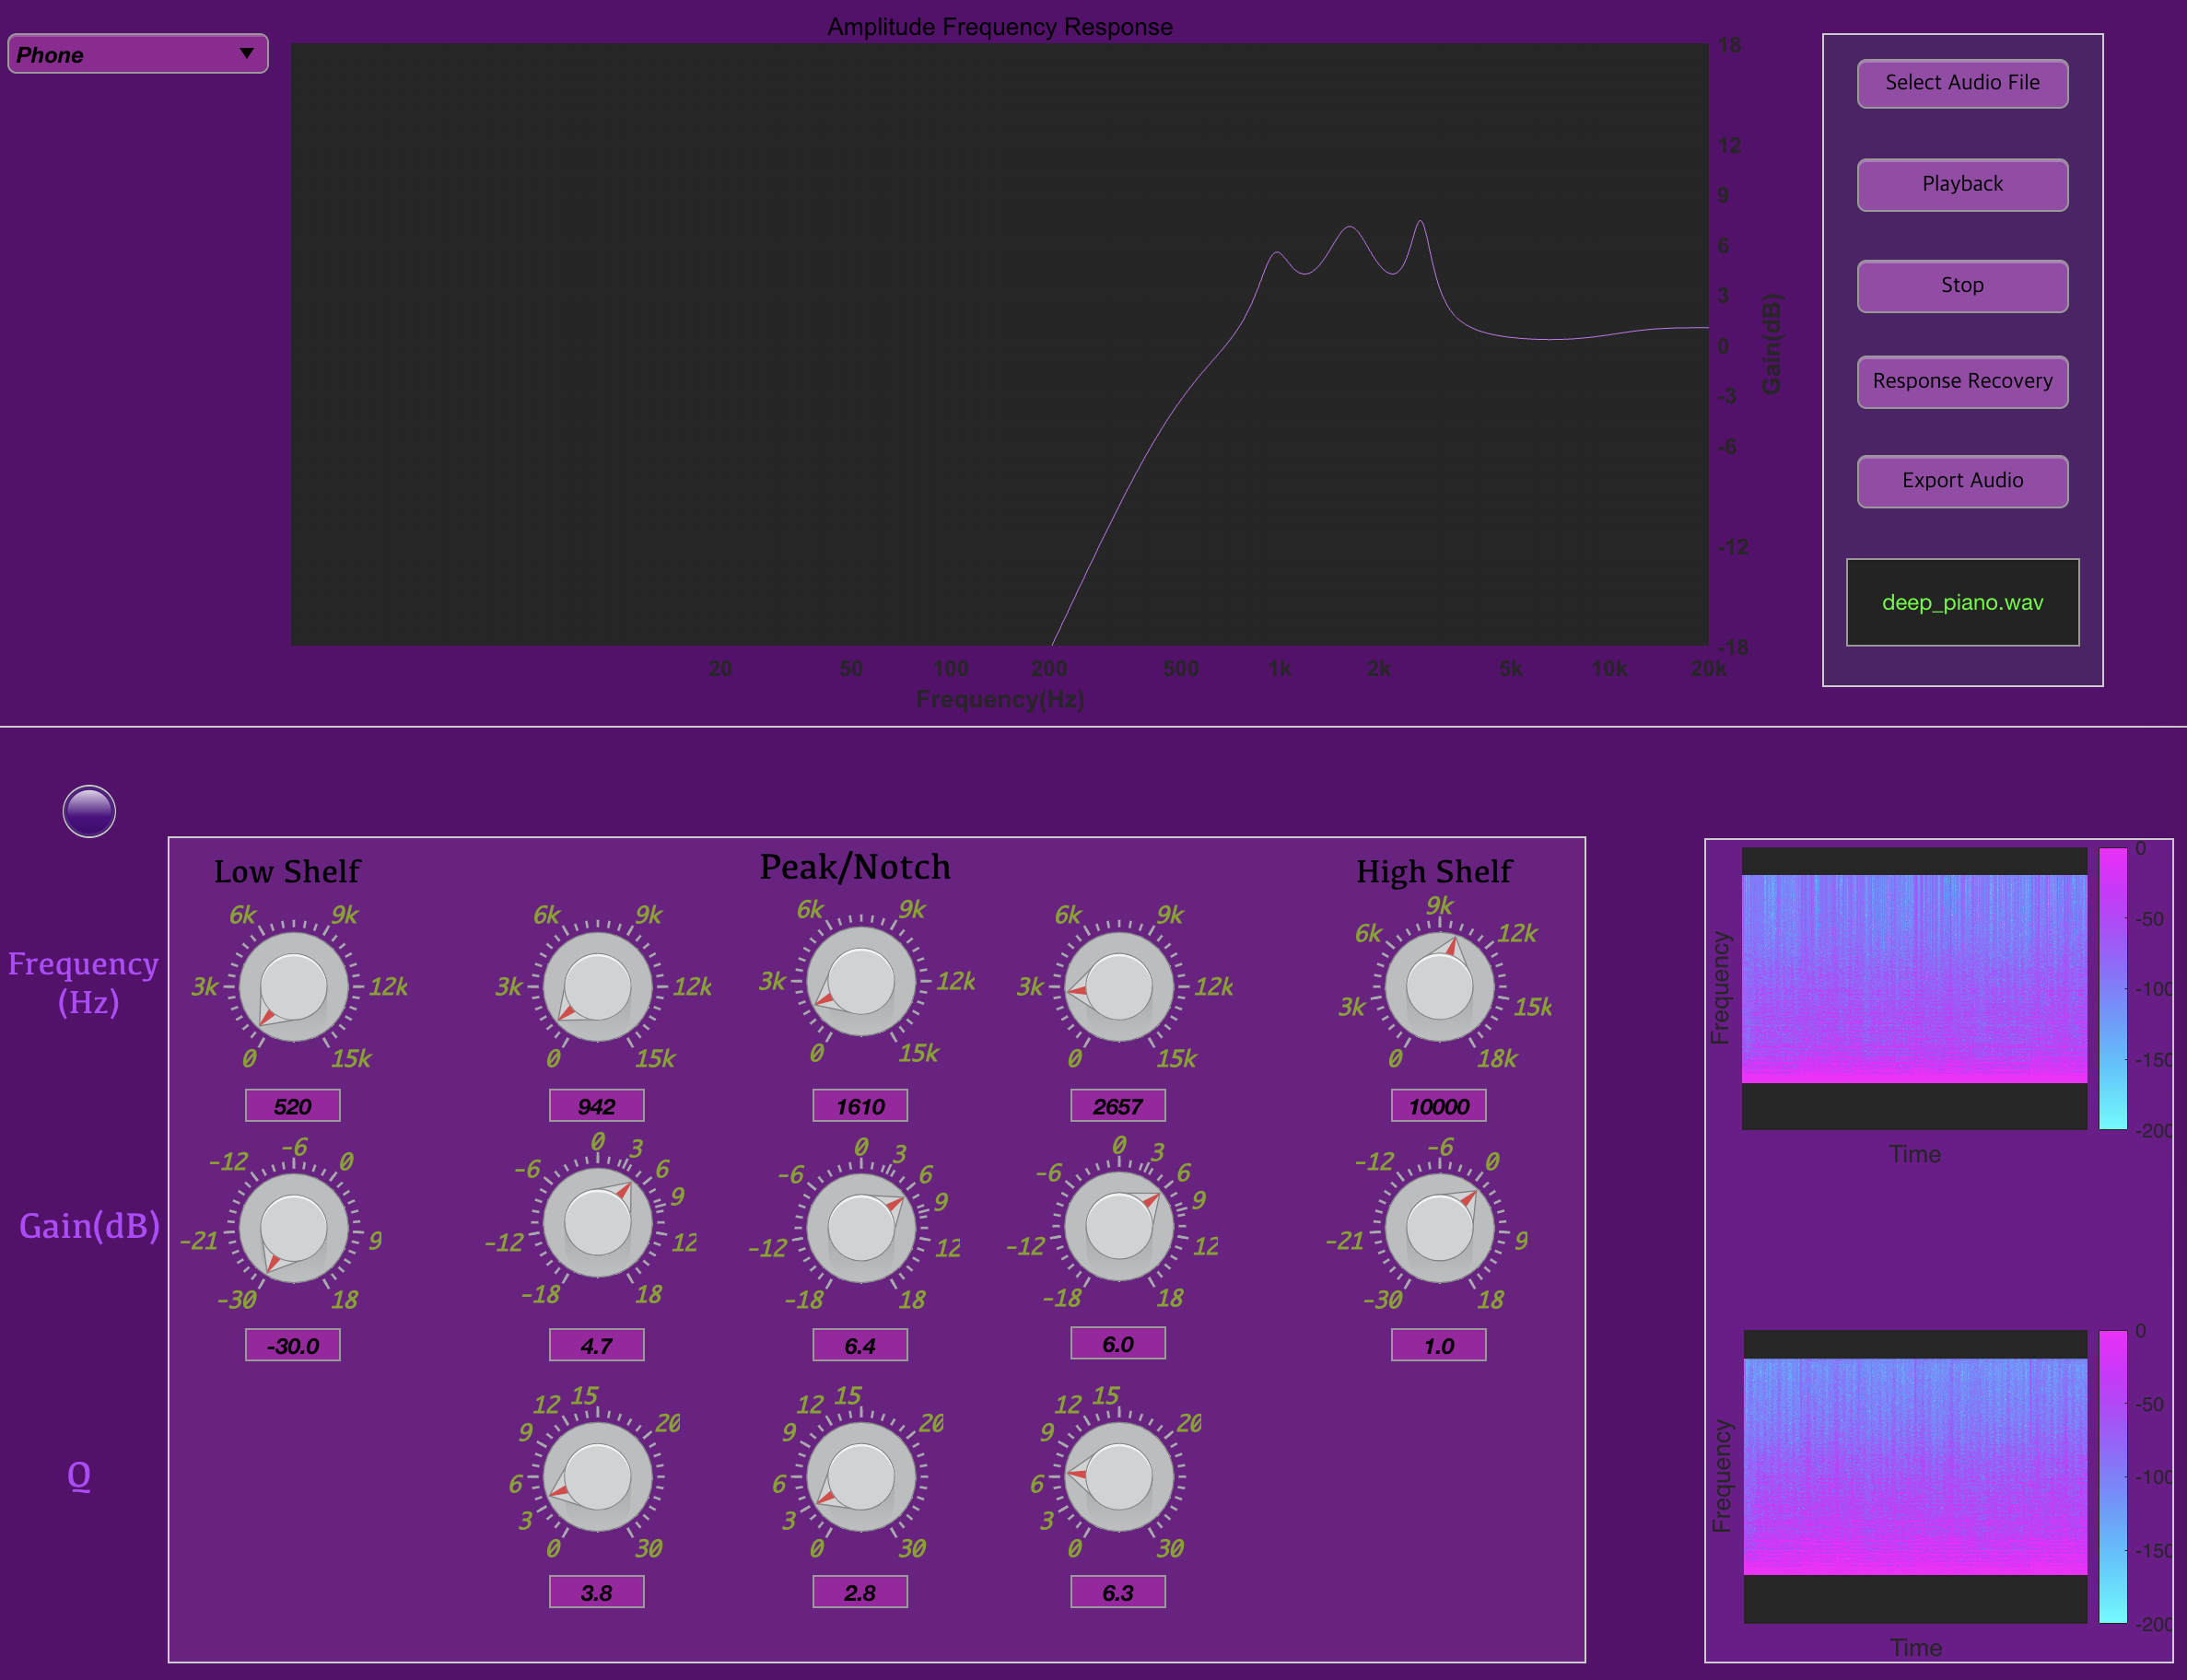
\includegraphics[width=2in]{Image/PhonePreset.png}
    }
    \subfigure['Above Enhance' preset]{
    	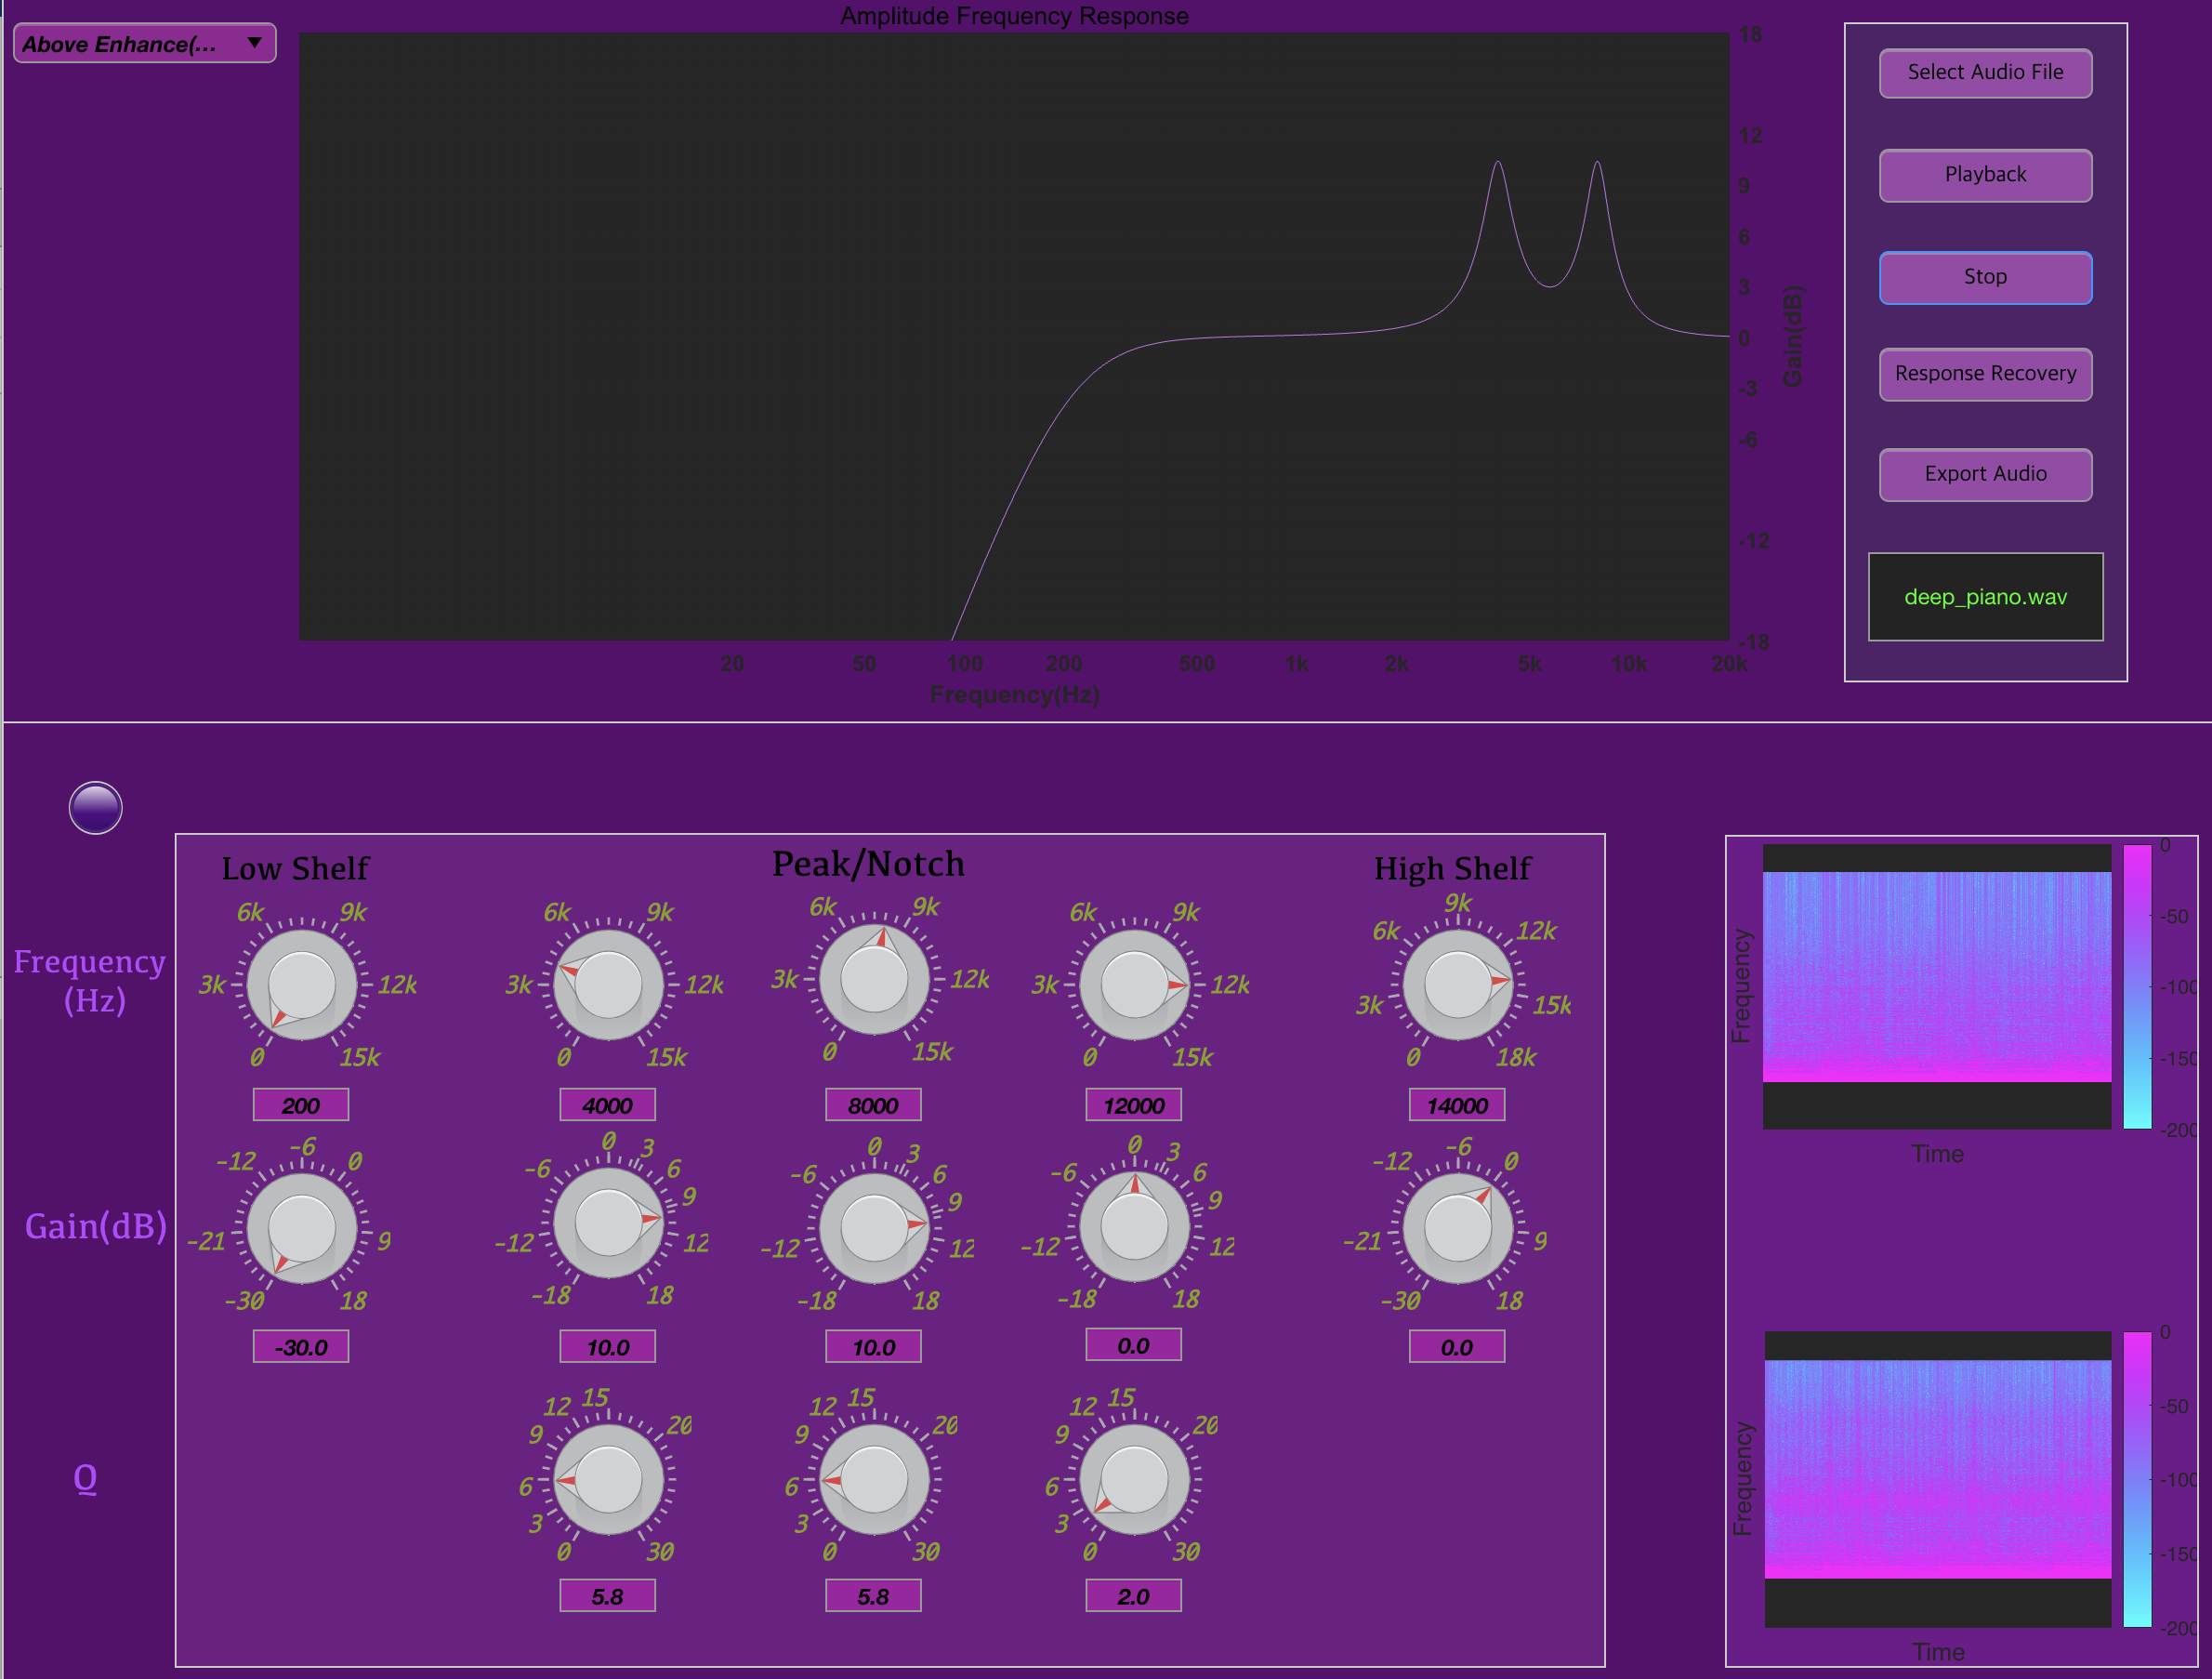
\includegraphics[width=2in]{Image/AboveEnhance.png}
    }
    \caption{Filter parameters adjustment, including sound optimization (above 2) and preset display (below 2).}
\end{figure}
%------------------------------------------------

\section{Phase Compensation}
As what has been discussed above, there is actually no strict phase compensation. So we can only find the optimal result by appropriating to the ideal compensation curve. To appropriate the target curve, some machine learning algorithms can be used to implement the phase compensation, such as genetic algorithm. 

The genetic algorithm is a method for solving both constrained and unconstrained optimization problems that is based on natural selection, the process that drives biological evolution. The genetic algorithm repeatedly modifies a population of individual solutions. At each step, the genetic algorithm selects individuals from the current population to be parents and uses them to produce the children for the next generation. Over successive generations, the population "evolves" toward an optimal solution. You can apply the genetic algorithm to solve a variety of optimization problems that are not well suited for standard optimization algorithms, including problems in which the objective function is discontinuous, nondifferentiable, stochastic, or highly non-linear. The genetic algorithm can address problems of mixed integer programming, where some components are restricted to be integer-valued\footnote{Matlab documentation, https://www.mathworks.com/help/gads/what-is-the-genetic-algorithm.html}.
\begin{figure}[h]
    \centering
	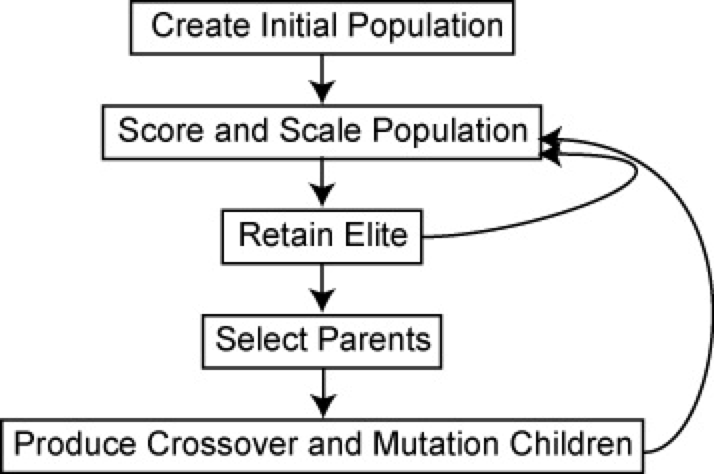
\includegraphics[width=2.5in]{Image/GeneticAlgorithmChart.png}
	\caption{The flow chart of genetic algorithm}
	\label{fig:textfig}
	\setfloatalignment{a} % Position the figure caption in the middle of the figure
\end{figure}

The genetic algorithm uses three main types of rules at each step to create the next generation from the current population:
\begin{enumerate}
    \item Selection rules select the individuals, called parents, that contribute to the population at the next generation. The selection is generally stochastic, and can depend on the individuals' scores.
    \item Crossover rules combine two parents to form children for the next generation.
    \item Mutation rules apply random changes to individual parents to form children.
\end{enumerate}

\begin{figure}[h]
    \centering
	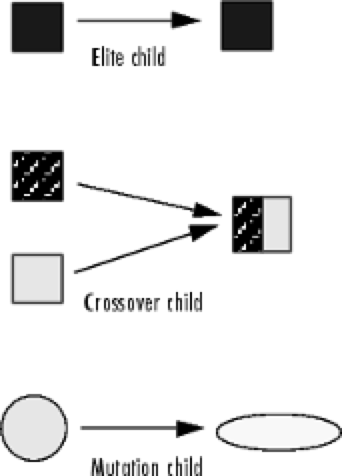
\includegraphics[width=1.5in]{Image/CreateNextGeneration.png}
	\caption{The flow chart of genetic algorithm}
	\label{fig:textfig}
	\setfloatalignment{a} % Position the figure caption in the middle of the figure
\end{figure}

In summary, the genetic algorithm is used to solve the optimization problems, which means that it can find parameters to appropriate the target curve, by transforming the problem into minimizing the difference between the actual curve and the target curve.

In this way, I design a first/second-order canonical low-pass filter and calculate its phase response, which is absolutely non-linear. Shown as in Figure 6 (a) and (b).
\begin{figure}[h!]
    \subfigure[First-order]{
        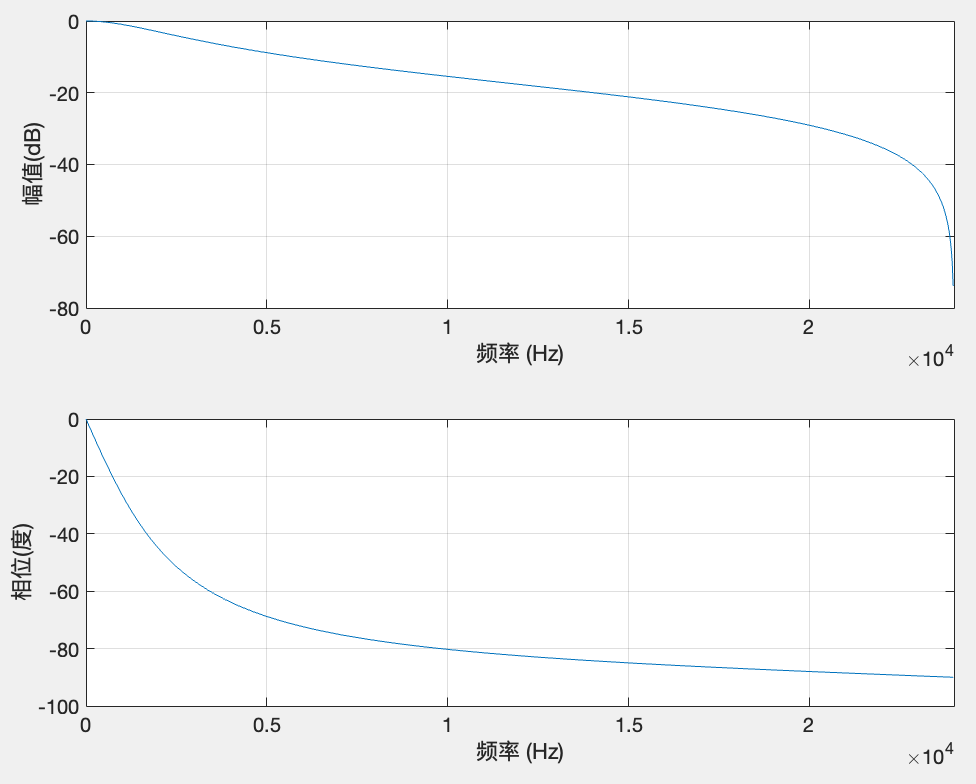
\includegraphics[width=2in]{Image/FirstOrderLowPassFilter.png}
    }
    \subfigure[Second-order]{
	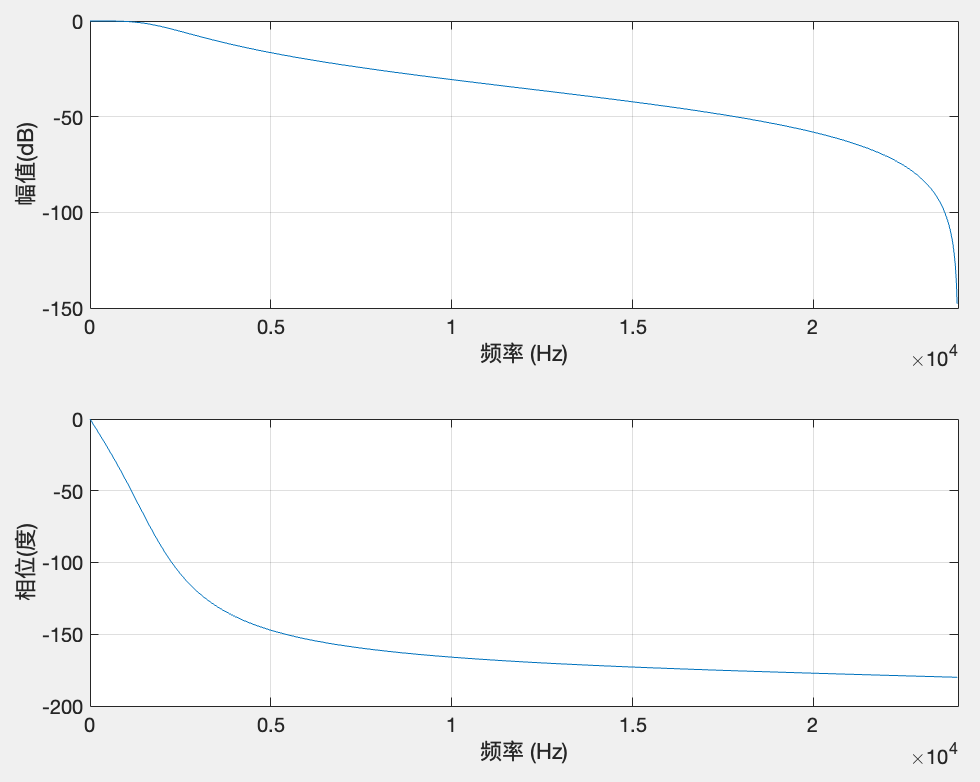
\includegraphics[width=2in]{Image/SecondOrderLowPassFilter.png}
    }
    \caption{Low-pass filter frequency(amplitude and phase) response}
\end{figure}
Then, I connect their phase response's zero and Nyquist frequency points as the ideal curve. Compute the difference between the ideal curve and the actual phase response curve as the compensation curve. As shown in Figure 7 (a) and (b).
\begin{figure}[h!]
    \subfigure[First-order]{
        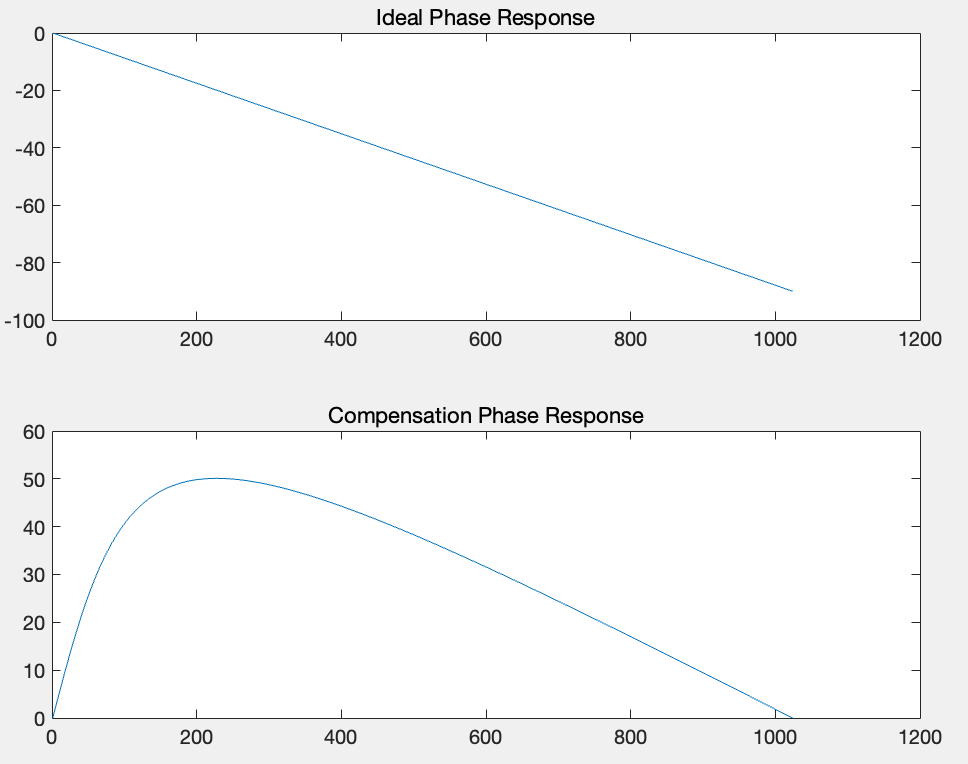
\includegraphics[width=2in]{Image/FirstOrderPhaseResponse.png}
    }
    \subfigure[Second-order]{
	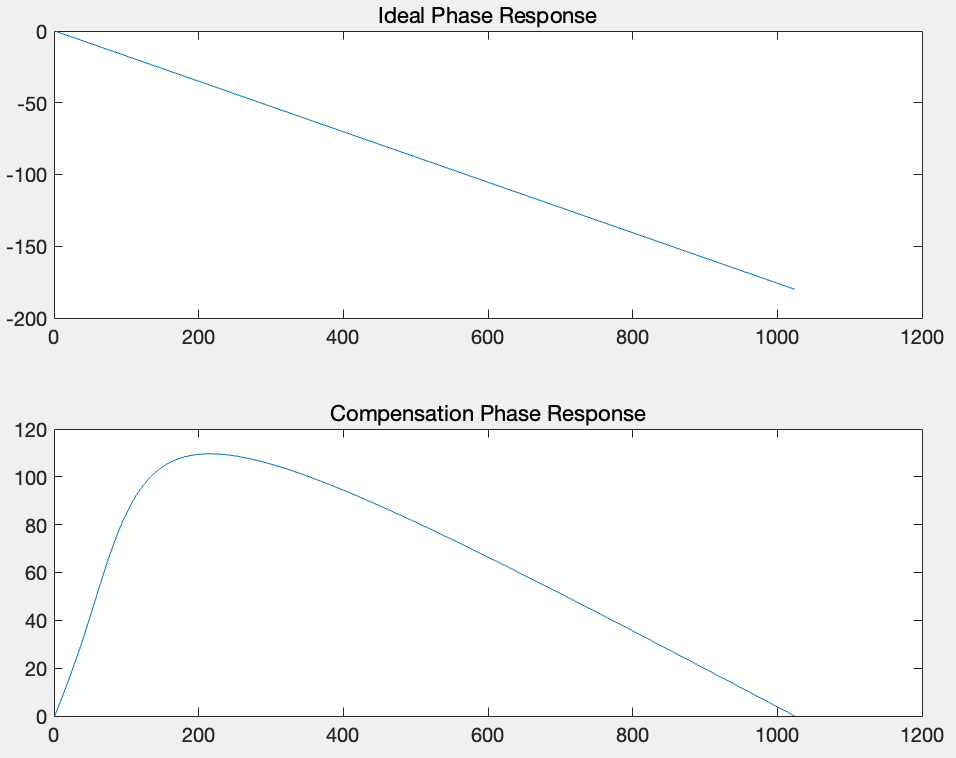
\includegraphics[width=2in]{Image/SecondOrderPhaseResponse.png}
    }
    \caption{Ideal and compensation curve}
\end{figure}

Matlab provides the implementation of genetic algorithm, which called function 'ga'. And function 'optimoptions' can be used to adjust the hyperparameters of genetic algorithm. Then the main task for me is to optimize the hyperparameters and obtain the compensation all-pass filter that best fits the linear phase response. I set the objective function of 'ga' as equation (2).
\begin{equation}
y=\sum_{i=1}^N{|x_{original}(i)-x_{traget}(i)|}
\end{equation}

In my opinion, the hyperparameter that dominates the training results is 'FunctionTolerance', which determines the stop point of genetic algorithm. If the average relative change in the best fitness function value over MaxStallGenerations generations is less than or equal to FunctionTolerance, the training will stop. Once the algorithm is run, the solver progresses will be shown as Figure 8.
\begin{figure}[h]
    \centering
	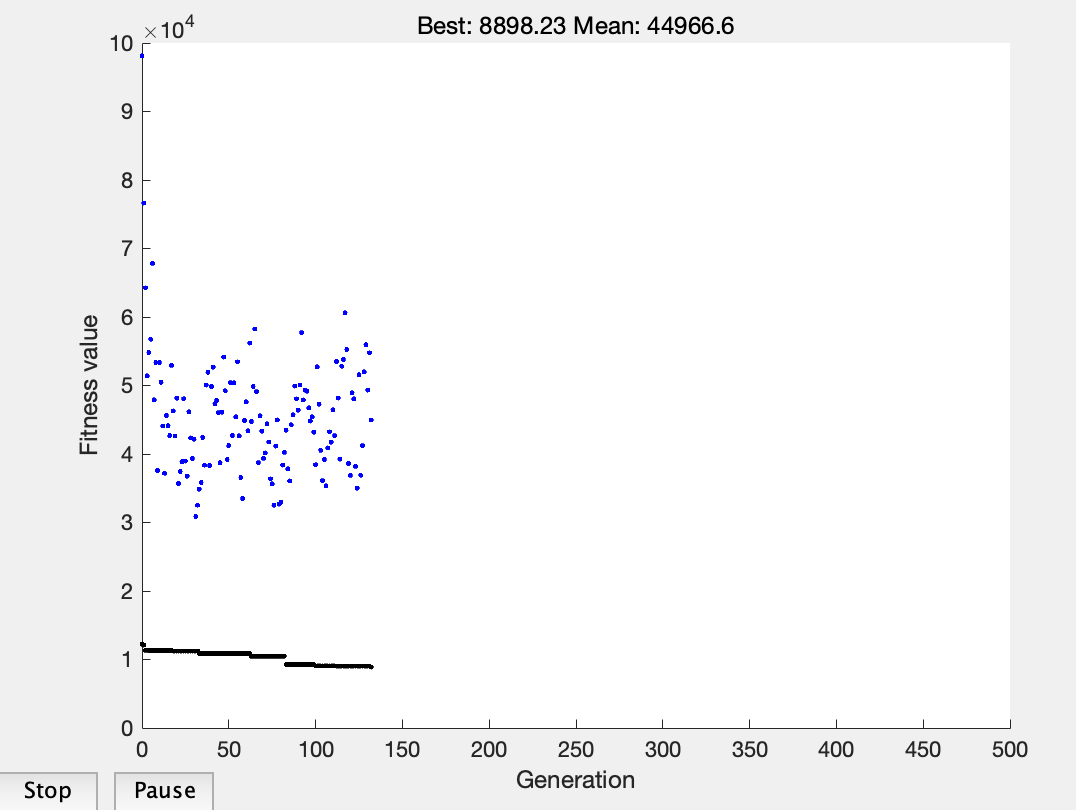
\includegraphics[width=3in]{Image/Generation.png}
	\caption{Solver progresses}
	\label{fig:textfig}
	\setfloatalignment{a} % Position the figure caption in the middle of the figure
\end{figure}

Hyperparameter is absolutely very import but cannot point to the only outcomes. Train the model multiple times is also essential. In this way, I obtain the best results of first/second-order low-pass filter compensation curve are shown as in Figure 9 (a) and (b). 
\begin{figure}[h!]
    \subfigure[First-order]{
        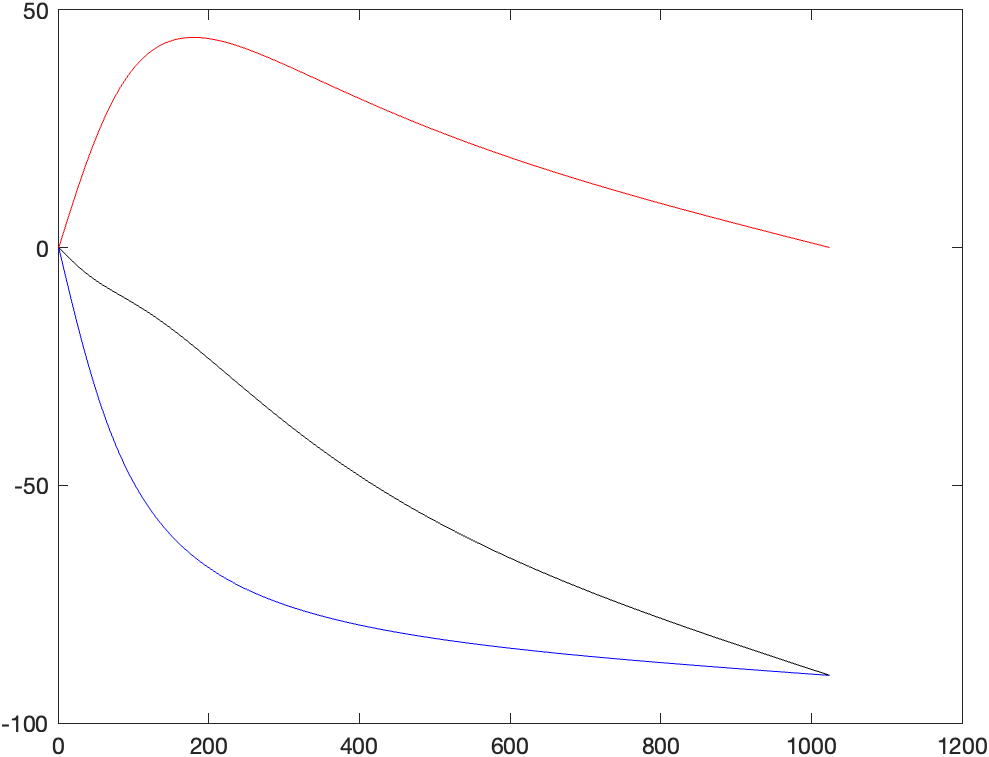
\includegraphics[width=2.2in]{Image/First-OrderCompensation.png}
    }
    \subfigure[Second-order]{
	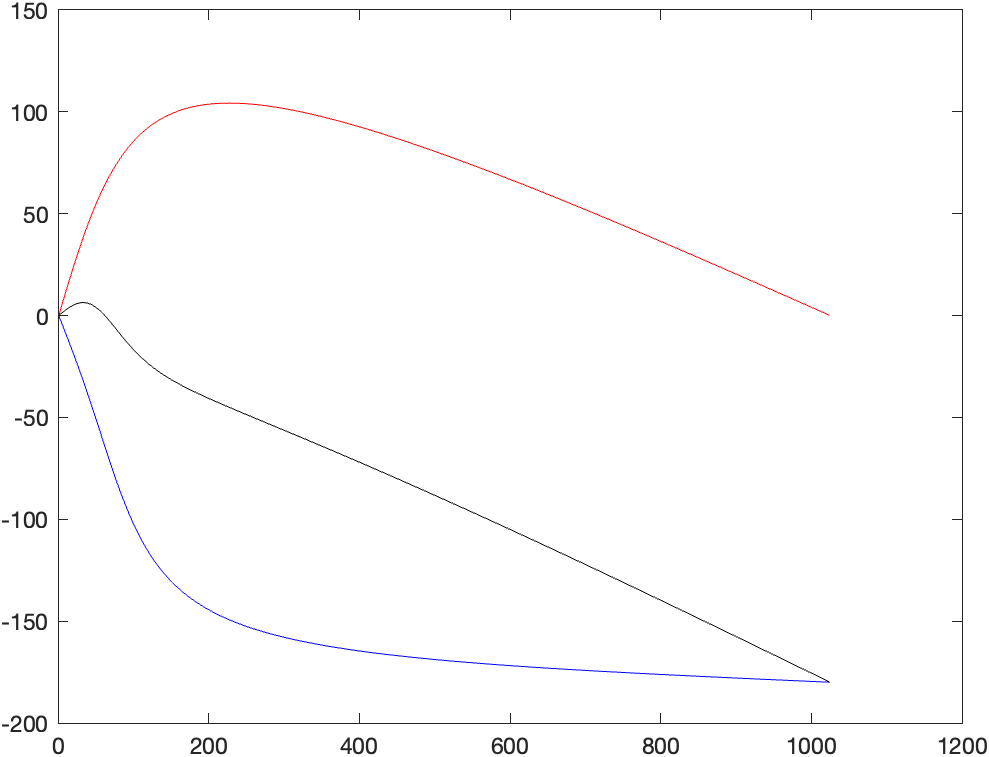
\includegraphics[width=2.2in]{Image/Second-OrderCompensation.png}
    }
    \caption{Compensation result}
\end{figure}
The hyperparameters of the above training results are all left in the matlab file.

As in Figure 9, the compensated first/second-order low-pass filters have approximate linear phase response. If we want to further fit the ideal curve, there are several possible ways:
\begin{itemize}
  \item Adjust the hyperparameters.
  \item Try different optimization algorithms, such as gradient descent method.
\end{itemize}
%------------------------------------------------

\section{Conclusion}
In this report, I adjust the parameters of the equalizer which was implemented in last term by myself, and implement the compensation to first/second-order low pass filter. For the further research, we may delve into the optimization problem of non-linear filter's phase compensation, including trying more different optimization algorithms.
Besides, this is my first time using LaTex finish the homework and I have tried my best to to make the layout of the report look better. Hope you like it and give me feedback to improve the whole report style. I would really appreciate for that.

\end{document}
